\documentclass[11pt, a4paper]{article}
\usepackage{graphicx}
\usepackage{float}
\usepackage[section]{placeins}
\graphicspath{{C:/Users/Nelson/Desktop/Harrisburg/CISC/Unit7/}}
\usepackage{listings}
\usepackage{url}
\usepackage[scaled=0.85]{beramono}
\renewcommand*\rmdefault{lmr}
\title{CISC 525-90-2016 - Unit 7\\ Hive Usage Report}
\author{Nelson Corrocher}
\date{August 2016}
\begin{document}
\maketitle
\section{Overview}
\paragraph{}This exercise is going to show some basic commands used in Hive and how it work. As a reminder, Hive is an interface to MapReduce so a similar output is expected. This exercise includes preparing a basic database in which tables can be created and data loaded. Then some simple select queries are going to be executed and its output exhibited. 

\paragraph{}The datasets used comes from a certain company. One dataset contains project information while the second table contains employee information. The two tables are joined by the Project Manager ID from the first table to its employee number on the second.

\paragraph{}One important note regarding the use of Hive is that its command interface is very frustrating. Instead of using it directly, most Hive SQL code was inputted in a text file and executed through \textbf{Hive -f 'filename'} command. 

\section{Creating the database} 
\paragraph{}A very simple database was created using the following command:
\begin{lstlisting}
CREATE DATABASE COMPANY_INFO;
\end{lstlisting}

\paragraph{}Note, this command was used directly in the console due to its simplicity.

\begin{figure}[H]
	\centering
	\fbox{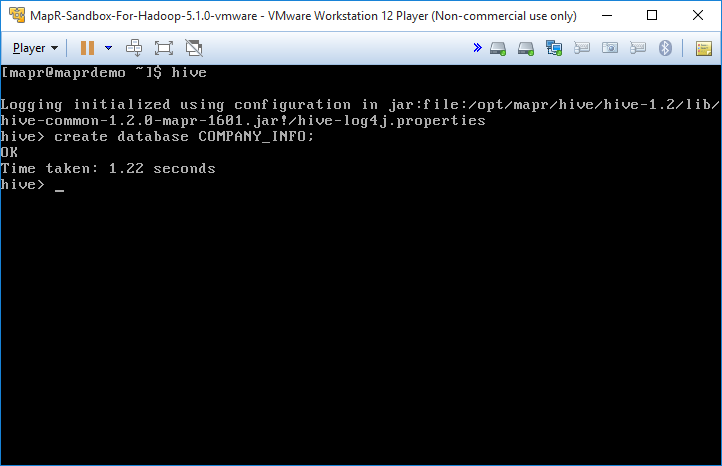
\includegraphics[width=1\textwidth]{create_database.png}}
	\caption{Database Creation Output}
\end{figure}

\section{Creating the tables}
\paragraph{}The queries themselves contain the data definition. 

\paragraph{}Table for Project Information: 
\begin{lstlisting}
CREATE TABLE PROJECT_INFO (
	PROJECT_NUMBER bigint COMMENT 'Project Primary Key',
	PM_ID bigint COMMENT 'Foreign Key in EMPLOYEE_INFO table',
	YTD_REVENUE double COMMENT 'Current Project Revenues')
ROW FORMAT DELIMITED
	FIELDS TERMINATED BY ','
	LINES TERMINATED BY '\n';
\end{lstlisting}

\paragraph{}Table for Employee Information: 
\begin{lstlisting}
CREATE TABLE EMPLOYEE_INFO (
	EMPLOYEE_NUMBER bigint COMMENT 'Employee Primary Key',
	FULL_NAME string COMMENT 'Employee Name',
	AGE int COMMENT 'in years',
	EMPLOYMENT_TIME int COMMENT 'in years')
ROW FORMAT DELIMITED
FIELDS TERMINATED BY ','
LINES TERMINATED BY '\n';
\end{lstlisting}

\paragraph{}Note: If the 'FIELDS' and 'LINES' statements are omitted, the loading data step fails and fills the table with only NULLs. This was not extensively tested, but is probably because the datasets were exported to CSVs using Excel, and thus, having DOS text format.

\begin{figure}[H]
	\centering
	\fbox{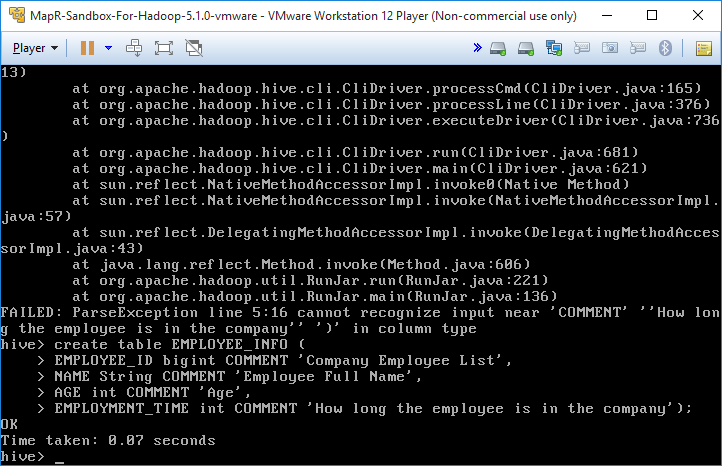
\includegraphics[width=1\textwidth]{create_table_example.png}}
	\caption{Table creation output example}
\end{figure}

\section{Loading the data}
\paragraph{}Loading data into PROJECT\_INFO table:
\begin{lstlisting}
LOAD DATA LOCAL INPATH '/home/mapr/prj.csv'INTO TABLE PROJECT_INFO;
\end{lstlisting}

\paragraph{}Loading data into EMPLOYEE\_INFO table:
\begin{lstlisting}
LOAD DATA LOCAL INPATH '/home/mapr/hr.csv'INTO TABLE EMPLOYEE_INFO;
\end{lstlisting}

\begin{figure}[H]
	\centering
	\fbox{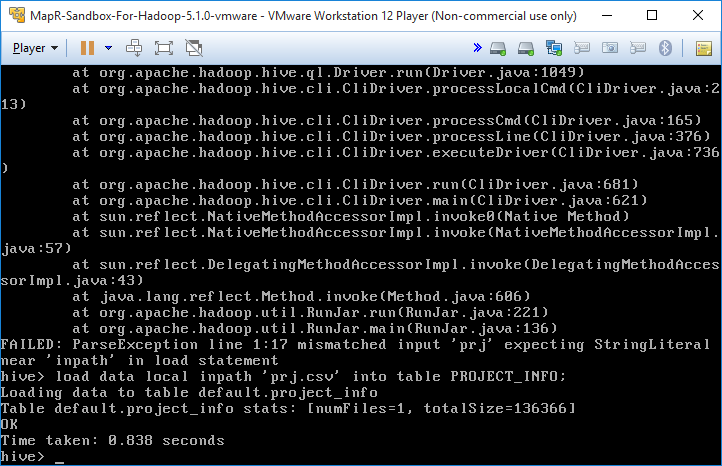
\includegraphics[width=1\textwidth]{loading_data_example.png}}
	\caption{Loading data example}
\end{figure}

\section{Running select queries for analysis}
\paragraph{}The select queries executed in Hive are compiled in MapReduce and then executed. This can be seen in the command prompt output. The first thing to be noticed is that all but basic select * from table query take a lot of time to run in comparison to regular RDBS.

\paragraph{}The first query executed was a simple test to see if the data was correctly imported. This SELECT statements was relatively fast and executed in 2.88 seconds. As mentioned in class, this happens because Hive directly extracts the data from table in these very simple queries.
\begin{lstlisting}
SELECT * FROM EMPLOYEE_INFO;
\end{lstlisting}

\begin{figure}[H]
	\centering
	\fbox{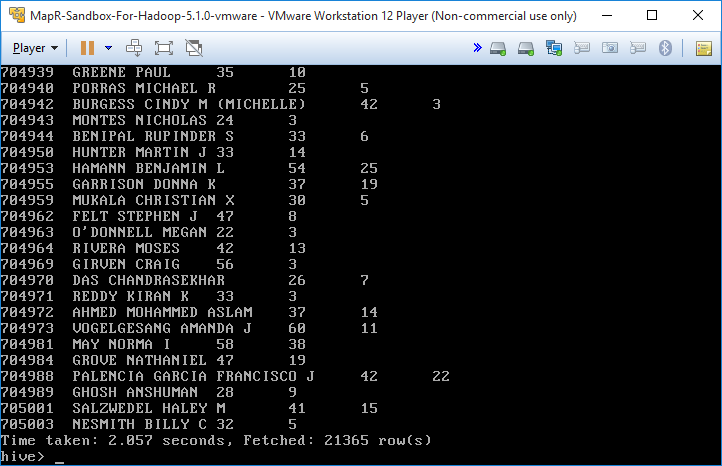
\includegraphics[width=1\textwidth]{select_statement_example.png}}
	\caption{Running a simple query}
\end{figure}

\paragraph{}The next query was just a SELECT SUM to test the results. One can notice that the execution time increased by a lot, due to Hive converting the query to MapReduce code and them running it in Hadoop. 
\begin{lstlisting}
SELECT SUM(YTD_REVENUE) FROM PROJECT_INFO;
\end{lstlisting}

\begin{figure}[H]
	\centering
	\fbox{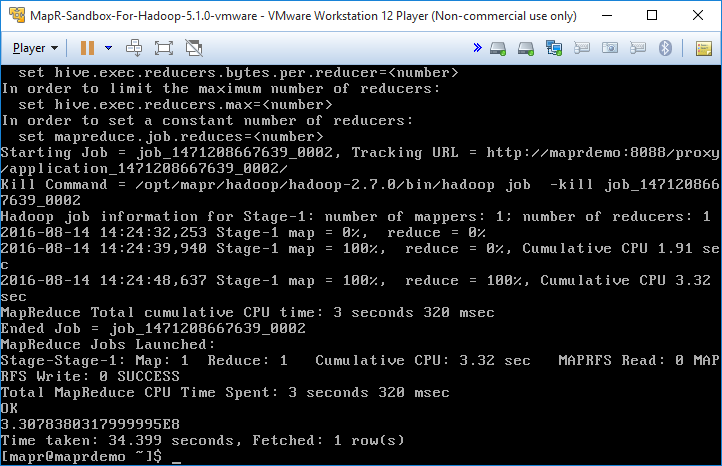
\includegraphics[width=1\textwidth]{select_sum_example.png}}
	\caption{Running an aggregation query}
\end{figure}

\paragraph{}The final test was to execute a JOIN query on the two tables. The time taken was not much higher than the SUM Query. This could imply that the overhead from Hadoop MapReduce framework is what really takes a lot of time in these queries.
\begin{lstlisting}
SELECT
	b.EMPLOYEE_NUMBER,
	b.FULL_NAME,
	sum(a.YTD_REVENUE)
FROM
	PROJECT_INFO a JOIN EMPLOYEE_INFO b
		ON (a.PM_ID = b.EMPLOYEE_NUMBER)
WHERE b.EMPLOYMENT_TIME < 10
GROUP BY
	b.EMPLOYEE_NUMBER,
	b.FULL_NAME;
\end{lstlisting}

\begin{figure}[H]
	\centering
	\fbox{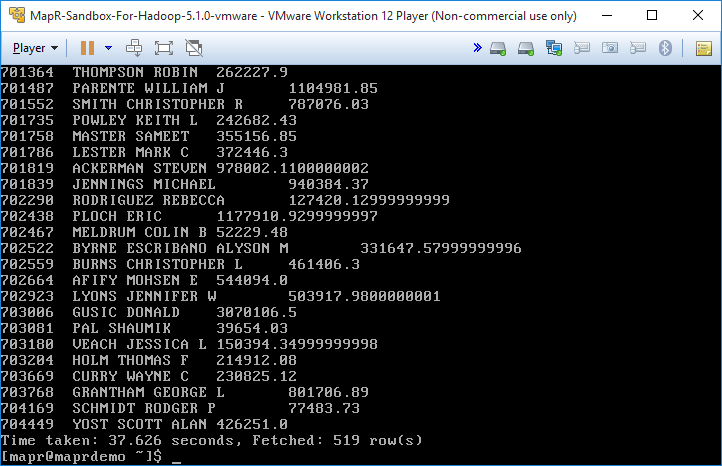
\includegraphics[width=1\textwidth]{select_joint_example.png}}
	\caption{Running a join query}
\end{figure}

\section{Conclusion}
\paragraph{}The command line interface for Hive is bad and very difficult to use for everything but the most simple queries. A better approach is to write the code in a text file and execute it through \textbf{Hive -f 'filename'}. The feel of Hive SQL is very similar to SQL, although it would be interesting to see if and how nested queries would work. Finally, the overhead of MapReduce framework is significant in comparison to regular RDBS. The real benefits of using Hive couldn't be tested due the environment having only one node and only test data.

\begin{thebibliography}{1}
Only the slides from class.
\end{thebibliography}

\paragraph{} Total words (excluding title and references): 797 words

\end{document}